\documentclass[12pt,a4paper]{amsart}
\usepackage[slovene, english]{babel}
\usepackage[utf8]{inputenc}
%\usepackage[T1]{fontenc}
\usepackage{amsmath,amssymb,amsfonts}
\usepackage[dvipsnames,usenames]{color}
\usepackage{algorithmicx,algpseudocode}
\usepackage{graphicx}
\usepackage{hyperref}


\textwidth 15cm
\textheight 24cm
\oddsidemargin.5cm
\evensidemargin.5cm
\topmargin-5mm
\addtolength{\footskip}{10pt}
\pagestyle{plain}

\overfullrule=15pt % oznaci predlogo vrstico

\newtheorem{definition}{Definition}[section]
\newtheorem{lemma}[definition]{Lemma}
\newtheorem{theorem}[definition]{Theorem}
\newtheorem{corollary}[definition]{Corollary}

\def\R{\mathbb R}
\def\N{\mathbb N}
\def\Z{\mathbb Z}
\def\C{\mathbb C}
\def\Q{\mathbb Q}

\begin{document}

\thispagestyle{empty}
\noindent{\large
University of Ljubljana \hfill  \today\\[1mm]
Faculty of Computer and Information Science  \\[5mm]
%IŠRM -- 2.~stopnja
}
%\vfill
\begin{center}{\large
Computational topology\\[4mm]
% Seminarska naloga\\[4mm]
{\bf Text classification using persistent homology}\\[4mm]
Matija Čufar, Domen Keglevič\\[6mm]
}
\end{center}
\bigskip

\section{Introduction}
Persistent homology is a method from topological data analysis which enables us
to calculate and compare features of topological spaces at different spatial
resolutions. Some features persist at wide range of spatial resolutions and are
more likely to represent the underlying space. This approach has been applied to
many different domains ranging from image analysis~\cite{nakane2015homology} to
genome studies~\cite{camara2016topological}.

In this seminar assignment we try to use persistence homology for text
classification. We pick four different text domains and try to distinguish
between them, based on their persistence diagrams.

\section{Methods}

We have chosen texts from the following domains:

\begin{itemize}
  \setlength\itemsep{0.5em}
\item Excerpts from the Old and New Testaments of the Bible,
\item articles from \url{phys.org},
\item recipes from \url{allrecipes.com}.
\end{itemize}

For each of the domains, we picked ten texts, each at least $100$ words long. We
used the Gudhi~\cite{maria2014gudhi}, a library for topological data analysis,
to compute persistent homology on the texts.

To compute the persistent homology of a data set, we first need to represent it
as a simplicial, or some other kind of complex. We used the following two
approaches to build simplicial complexes for each of the domains:

\subsection{Feature based approach}

In our first approach we associated each text with a point in $\R ^6$. Each
dimension was representing one of text features. We used the following features:
\begin{itemize}
  \setlength\itemsep{0.5em}
  \item the ratio of (average word length)/(longest word length),
  \item the ratio of (average sentence length)/(longest sentence length),
  \item the ratio of the total number of three words with the highest tf-idf
    value among all the words,
  \item the ratio of the number of words of length $\le 8$ among all words,
  \item the ratio of the number of words of length $\ge 9$ among all words.
  \item the ratio of (number of different words)/(number of all words)
\end{itemize}

Note that all features are normalized in order to avoid giving too much weight
to those that would have large size otherwise.
After computing features and mapping texts to points in $\R ^6$ we
built Alpha and Vietoris-Rips complexes on each of the domains.

\subsection{Distribution based approach}

Our second approach involved computing distributions of word and sentence
lengths. This gives us two distributions for each text. Two distributions of the
same type (word or sentence) were then compared using the following distance
measures:

\begin{itemize}
\item The Hellinger distance:

\begin{equation*}
  H(P,Q) = \sqrt{\frac{1}{2} \sum_{i=1}^k\left(\sqrt{p_i} -
    \sqrt{q_i}\right)^2}\ ,
\end{equation*}

\item the Chi-squared distance:

\begin{equation*}
  \chi^2(P,Q) = \frac{1}{2}\sum _{i=1}^n\frac{(p_i - q_i)^2}{(p_i + q_i + \varepsilon)}\ ,
\end{equation*}

\item the Euclidean distance:

\begin{equation*}
  E(P,Q) = \sqrt{\sum_{i=1}^k\left(p_i - q_i\right)^2}\ ,
\end{equation*}
\end{itemize}

\noindent
where $P$ and $Q$ are the discrete distributions and $p_i$ and $q_i$ are the
$i$-th bins of corresponding distributions. The $\varepsilon$ in the Chi-squared
distance is a small positive constant used to avoid dividing by zero.

We used these distances to compute distance matrix for each of the
domains and used distance matrices to build Vietoris-Rips complexes.

\subsection{Domain comparison}

When the simplicial complexes were built, we calculated persistence diagrams for
each complex and computed the bottleneck distances between them. We expected the
distances would help us distinguish between the texts. For example, the distance
between the texts taken from the Bible should be smaller than the rest.

\section{Results}

\subsection{Feature based approach} Bottleneck
distance matrix for the Alpha complex is shown in Table~\ref{tab:alpha}.
Barcode plots are shown in Figure~\ref{fig:barcode:alpha}.

As we can see from the distance matrix, the method did not produce meaningful
results. The first thing we notice is that all the distances are very small,
with the highest being only $0.008$. Other examples that show the
ineffectiveness of this method are the fact that the Old Testament differs the
most from the New Testament and the fact that according to this method, physics
article abstracts are very similar to recipes.

Something we notice from the barcode plots is that recipes appear to have some
persistent four-dimensional features. These features could be used to
distinguish recipes from other texts, but we are not sure they would appear in
other recipe datasets.

Results for the Vietoris-Rips complex are similar to the results for Alpha
complex, so will skip their presentation.

\begin{table}
  \centering
  \begin{tabular}{c|cccc}
                  & Old Testament & New Testament & phys.org & recipes \\ \hline
    Old Testament & $0.000$ & $0.008$ & $0.003$ & $0.003$ \\
    New Testament & $0.008$ & $0.000$ & $0.008$ & $0.008$ \\
    phys.org      & $0.003$ & $0.008$ & $0.000$ & $0.002$ \\
    recipes       & $0.003$ & $0.008$ & $0.002$ & $0.000$ \\
  \end{tabular}

  \caption{The distance matrix calculated from the Alpha complexes.}
  \label{tab:alpha}
\end{table}

\begin{figure}
  \centering
  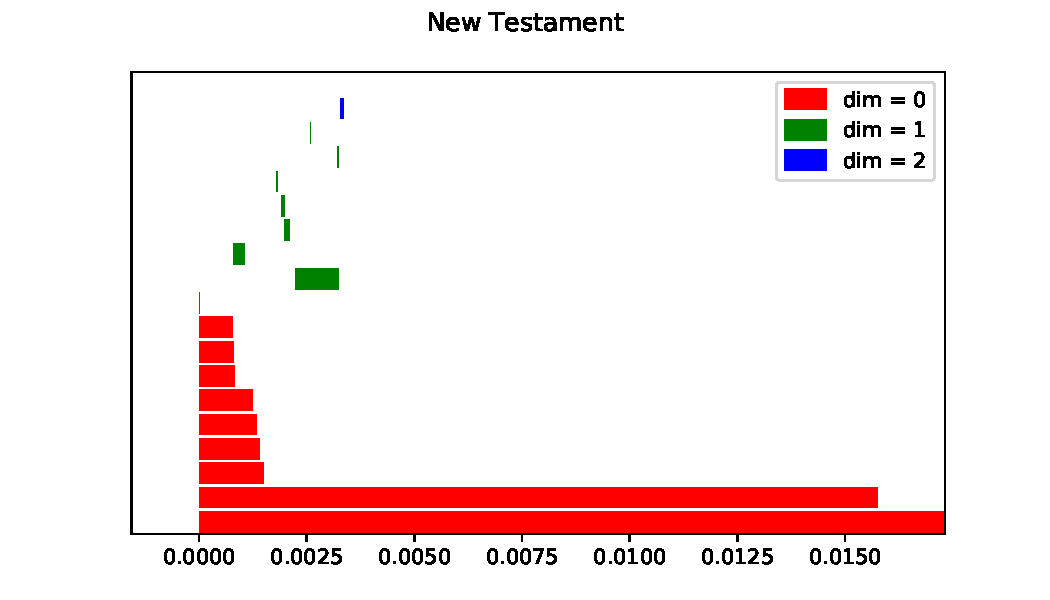
\includegraphics[width=0.45\textwidth]{../plots/barcodes/bible-new-alpha}
  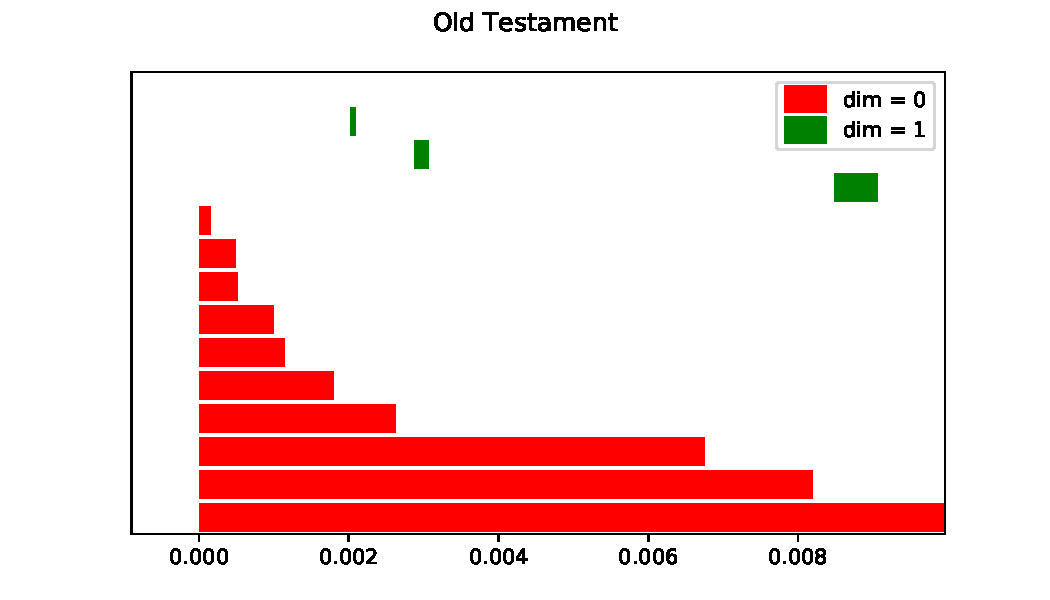
\includegraphics[width=0.45\textwidth]{../plots/barcodes/bible-old-alpha}
  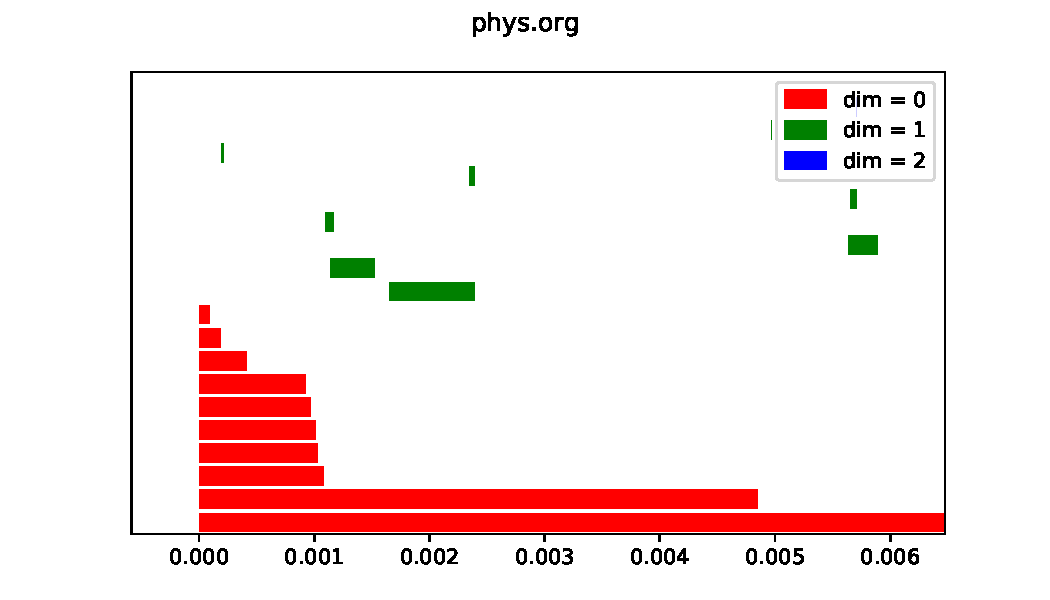
\includegraphics[width=0.45\textwidth]{../plots/barcodes/phys-alpha}
  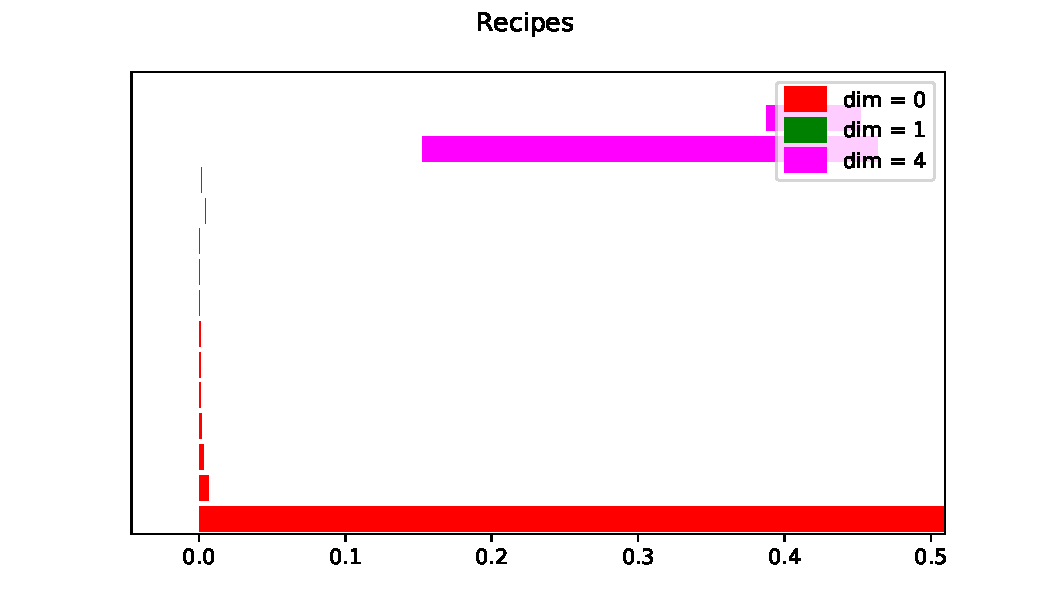
\includegraphics[width=0.45\textwidth]{../plots/barcodes/recipes-alpha}
  \caption{Persistence barcodes of the domains, calculated from the Alpha
    complexes.}
  \label{fig:barcode:alpha}
\end{figure}

\subsection{Distribution based approach}

The best results using the distribution dist-ance-based method were given by the
Hellinger and Chi-squared distances between the distributions of sentence
lengths. The distance matrices are presented in Tables~\ref{tab:hell}
and~\ref{tab:chi} and the persistence barcodes for the Hellinger distance are
shown in Figure~\ref{fig:barcode:hell}.

We see from the tables, that according to these methods, the texts taken from
the Bible are the most similar among each other and that recipes differ the most
from other domains. Physics articles are somewhere in between. These are the
results we expected, but perhaps it's worth pointing out that the distances
between the texts are still very small and that out of all eight different ways
of classifying the texts we tried, only these two produced meaningful
results. Perhaps these methods only work with these specific datasets and should
be double-checked with other text domains before drawing conclusions.

\begin{table}
  \centering
  \begin{tabular}{r|cccc}
                  & Old Testament & New Testament & phys.org & recipes \\ \hline
    Old Testament & 0.000 & 0.015 & 0.040 & 0.112 \\
    New Testament & 0.015 & 0.000 & 0.033 & 0.103 \\
    phys.org      & 0.040 & 0.033 & 0.000 & 0.105 \\
    recipes       & 0.112 & 0.103 & 0.105 & 0.000 \\
  \end{tabular}

  \caption{The distance matrix calculated from the Vietoris-Rips complexes,
    built using the Hellinger distance between sentence length distributions.}
  \label{tab:hell}
\end{table}

\begin{table}
  \centering
  \begin{tabular}{r|cccc}
                  & Old Testament & New Testament & phys.org & recipes \\ \hline
    Old Testament & 0.000 & 0.031 & 0.078 & 0.193 \\
    New Testament & 0.031 & 0.000 & 0.060 & 0.166 \\
    phys.org      & 0.078 & 0.060 & 0.000 & 0.154 \\
    recipes       & 0.193 & 0.166 & 0.154 & 0.000 \\
  \end{tabular}
  \caption{The distance matrix calculated from the Vietoris-Rips complexes,
    built using the Chi-squared distance between sentence length distributions.}
  \label{tab:chi}
\end{table}

\begin{figure}
  \centering
  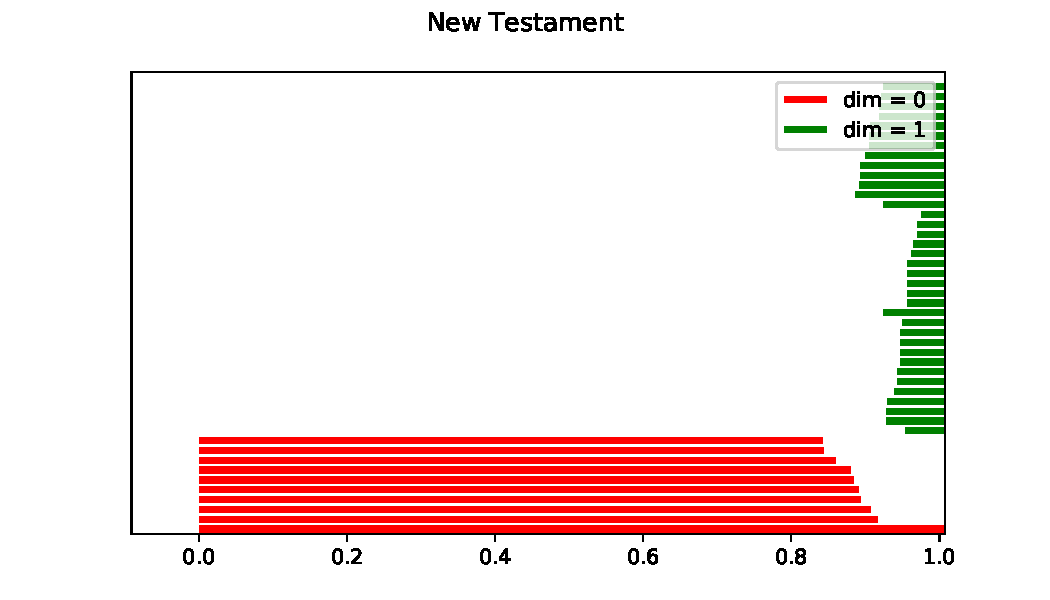
\includegraphics[width=0.45\textwidth]{../plots/barcodes/bible-new-hell}
  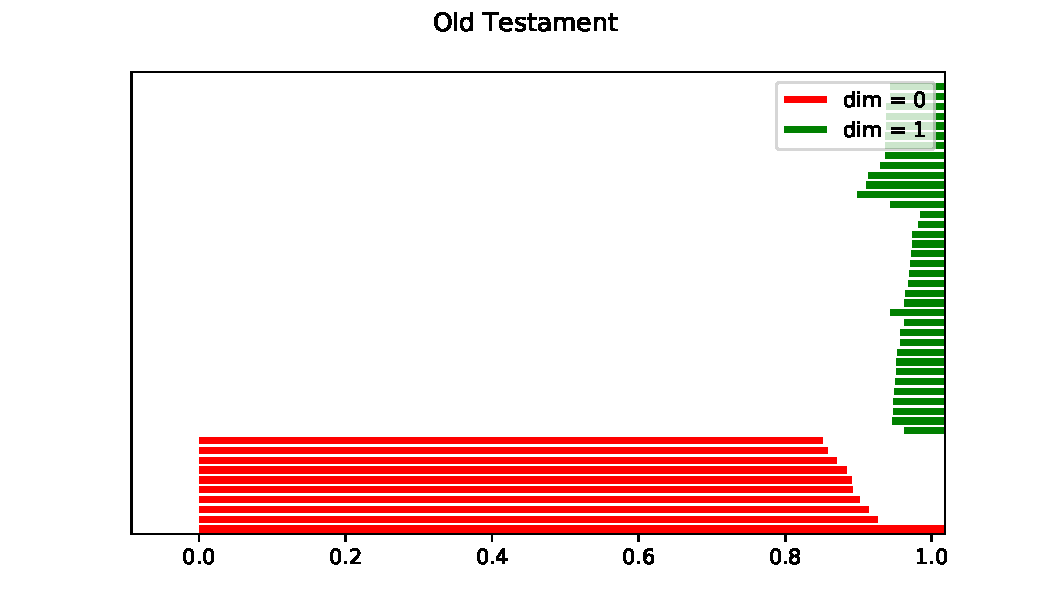
\includegraphics[width=0.45\textwidth]{../plots/barcodes/bible-old-hell}
  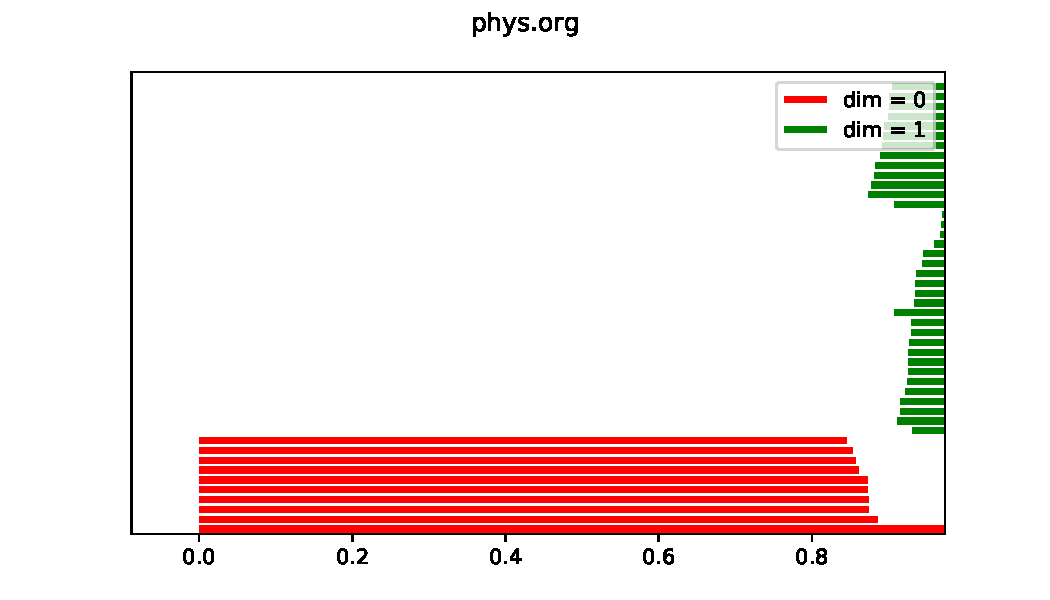
\includegraphics[width=0.45\textwidth]{../plots/barcodes/phys-hell}
  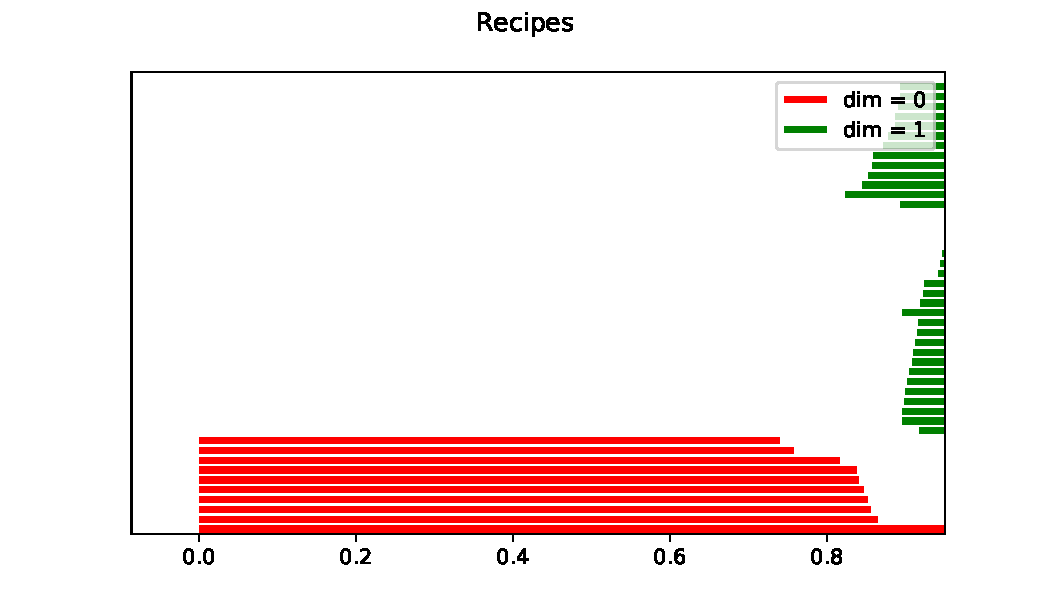
\includegraphics[width=0.45\textwidth]{../plots/barcodes/recipes-hell}
  \caption{Persistence barcodes of the domains, calculated from the
    Vietoris-Rips complexes, built using the Hellinger distance between sentence
    length distributions.}
  \label{fig:barcode:hell}
\end{figure}

\section{Conclusion}

We have attempted to classify text domains using persistent homology. Out of the
two approaches we used, the feature-based approach was incapable of
distinguishing between the domains. While using distances between sentence
length distributions showed some potential, it didn't convince us, considering
the fact that we used domains that have almost nothing in common and that the
detected distances were rather small.

Perhaps, the results would be better and more robust if we tried using a larger
number of texts for each domain and a larger number of domains. The method
should also be tested against domains that have more in common, for example,
scientific articles from different fields.

\section{Authors contributions}
Both authors have contributed to most parts of the seminar work. The exception
being that Domen prepared most of the presentation and Matija wrote most of the
report. Detailed contributions can be seen in commit history of GitHub
repository \url{https://github.com/dkegle/rt201617} which also contains all of
the code and data.

% biblio
\bibliographystyle{plain}
\bibliography{biblio}

% [2] Image analysis: https://www.ncbi.nlm.nih.gov/pmc/articles/PMC4448533/
% [3] Genome-wide maps: http://www.cell.com/cell-systems/pdf/S2405-4712(16)30183-1.pdf

\end{document}
